\documentclass[11pt]{article}

\usepackage[margin=1in]{geometry}
\usepackage{amsmath}
\usepackage{booktabs}
\usepackage{siunitx}
\usepackage{pgfplots}
\pgfplotsset{compat=1.18}
\usetikzlibrary{decorations.pathmorphing}

\title{How a Cup of Coffee Cools}
\author{A. Barista}
\date{}

\begin{document}
\maketitle

\begin{abstract}
  We derive Newton's law of cooling from a simple heat-balance argument and
  use it to model a cooling cup of coffee. Temperature curves are plotted
  for several starting temperatures, and the time until the coffee reaches
  a drinkable temperature is tabulated, including the effect of stirring
  in milk immediately after pouring.
\end{abstract}

\section{Introduction}

Anyone who has poured a fresh cup of coffee knows the routine: it is too hot
to drink at first, and after some waiting it settles into a pleasant,
drinkable temperature. This note works out the physics behind that cooling
process. We derive Newton's law of cooling from a simple heat-balance
argument \cite{newton1701}, solve the resulting differential equation, and
use the solution to predict how long a cup of coffee poured at different
starting temperatures takes to become drinkable. The exponential model used
here, and the typical cooling rates for a cup of coffee in still air, follow
the treatment of Vollmer \cite{vollmer2009}.

\section{Deriving Newton's law of cooling}

Consider a cup of coffee with temperature $T(t)$, surrounded by air at
constant ambient temperature $T_{\text{env}}$. Figure~\ref{fig:heat-paths}
sketches the three routes by which it loses heat: conduction through the
mug wall, and convection and evaporation from the free surface. All three
routes carry heat away faster the hotter the coffee is relative to its
surroundings, and radiation from the surface behaves the same way. When $T$
is not too far from $T_{\text{env}}$, their combined effect is well
approximated by a single heat-loss rate proportional to the temperature
difference between the coffee and its surroundings. That is, the rate at
which heat $Q$ leaves the coffee obeys

\begin{figure}[htb]
  \centering
  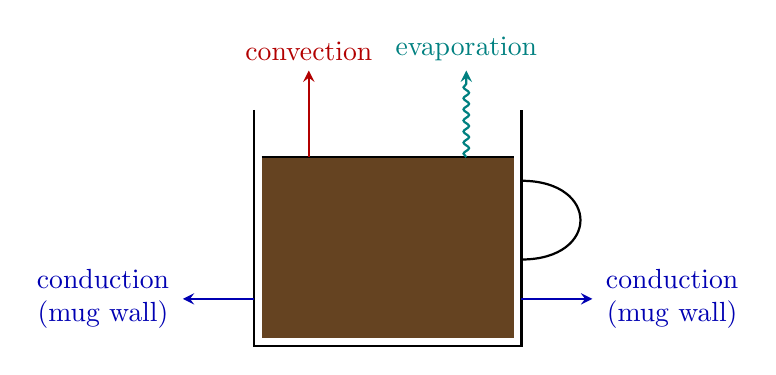
\begin{tikzpicture}[>=stealth]
    \definecolor{coffeebrown}{RGB}{101,67,33}

    % mug: left wall, bottom, right wall (open top)
    \draw[thick] (-1.7,3) -- (-1.7,0) -- (1.7,0) -- (1.7,3);
    % handle
    \draw[thick] (1.7,1.1) .. controls (2.7,1.1) and (2.7,2.1) .. (1.7,2.1);

    % coffee fill, below the rim
    \fill[coffeebrown] (-1.6,0.1) -- (-1.6,2.4) -- (1.6,2.4) -- (1.6,0.1) -- cycle;
    \draw[thick] (-1.6,2.4) -- (1.6,2.4);

    % conduction through the walls
    \draw[->, thick, blue!70!black] (-1.7,0.6) -- (-2.6,0.6);
    \node[left, blue!70!black, align=center] at (-2.65,0.6) {conduction\\(mug wall)};
    \draw[->, thick, blue!70!black] (1.7,0.6) -- (2.6,0.6);
    \node[right, blue!70!black, align=center] at (2.65,0.6) {conduction\\(mug wall)};

    % convection from the free surface
    \draw[->, thick, red!70!black] (-1.0,2.4) -- (-1.0,3.5);
    \node[above, red!70!black] at (-1.0,3.5) {convection};

    % evaporation from the free surface
    \draw[->, thick, teal, decorate,
      decoration={snake, amplitude=1pt, segment length=4pt, post length=3pt}]
      (1.0,2.4) -- (1.0,3.5);
    \node[above, teal] at (1.0,3.5) {evaporation};
  \end{tikzpicture}
  \caption{Heat leaving a cup of coffee: conduction through the mug wall,
    and convection and evaporation from the free surface. Radiation from
    the free surface (not shown) follows the same outward path as
    convection.}
  \label{fig:heat-paths}
\end{figure}
\begin{equation}
  \frac{dQ}{dt} = -h A \bigl(T(t) - T_{\text{env}}\bigr),
\end{equation}
where $h$ is an effective heat-transfer coefficient and $A$ is the exposed
surface area of the coffee (cup walls plus free surface). Since the coffee
has heat capacity $C = mc$ (mass times specific heat), $dQ = C\,dT$, so
\begin{equation}
  C \frac{dT}{dt} = -h A \bigl(T(t) - T_{\text{env}}\bigr).
\end{equation}
Collecting the constants $h$, $A$, and $C$ into a single cooling-rate
constant $k = hA/C > 0$ gives Newton's law of cooling in its familiar form:
\begin{equation}
  \label{eq:newton}
  \frac{dT}{dt} = -k\bigl(T(t) - T_{\text{env}}\bigr).
\end{equation}

Equation~\eqref{eq:newton} is a linear, first-order ODE. Writing
$u(t) = T(t) - T_{\text{env}}$ turns it into $\dot u = -ku$, whose solution
is $u(t) = u(0) e^{-kt}$. Substituting back, and writing $T_0 = T(0)$ for
the initial temperature, gives
\begin{equation}
  \label{eq:solution}
  T(t) = T_{\text{env}} + \bigl(T_0 - T_{\text{env}}\bigr) e^{-kt}.
\end{equation}

This is the exponential cooling curve: the coffee approaches room
temperature exponentially, with time constant $1/k$, regardless of how hot
it started. Equation~\eqref{eq:solution} is the form we use below to model
a real cup of coffee.

\section{A worked example}

\begin{figure}[t]
  \centering
  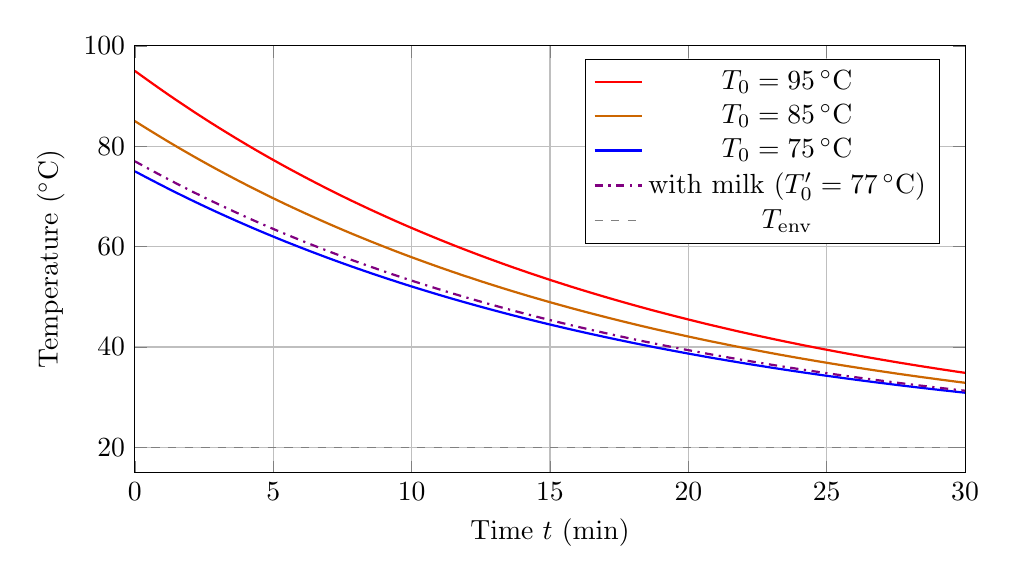
\begin{tikzpicture}
    \begin{axis}[
        width=\textwidth,
        height=7cm,
        xlabel={Time $t$ (min)},
        ylabel={Temperature (\si{\celsius})},
        xmin=0, xmax=30,
        ymin=15, ymax=100,
        legend pos=north east,
        grid=major,
      ]
      \addplot[thick, red, domain=0:30, samples=100]
        {20 + (95-20)*exp(-0.054*x)};
      \addlegendentry{$T_0 = \SI{95}{\celsius}$}
      \addplot[thick, orange!80!black, domain=0:30, samples=100]
        {20 + (85-20)*exp(-0.054*x)};
      \addlegendentry{$T_0 = \SI{85}{\celsius}$}
      \addplot[thick, blue, domain=0:30, samples=100]
        {20 + (75-20)*exp(-0.054*x)};
      \addlegendentry{$T_0 = \SI{75}{\celsius}$}
      \addplot[thick, dash dot, violet, domain=0:30, samples=100]
        {20 + (77-20)*exp(-0.054*x)};
      \addlegendentry{with milk ($T_0' = \SI{77}{\celsius}$)}
      \addplot[dashed, gray, domain=0:30, samples=2] {20};
      \addlegendentry{$T_{\text{env}}$}
    \end{axis}
  \end{tikzpicture}
  \caption{Coffee temperature versus time: three starting temperatures for
    black coffee, from Equation~\eqref{eq:solution} with
    $T_{\text{env}} = \SI{20}{\celsius}$ and $k = \SI{0.054}{\per\minute}$,
    plus one curve for coffee poured at \SI{85}{\celsius} with milk
    stirred in immediately, dropping it to $T_0' = \SI{77}{\celsius}$ by
    Equation~\eqref{eq:mixing}. All curves decay toward room temperature
    with the same time constant $1/k \approx \SI{18.5}{\minute}$.}
  \label{fig:cooling}
\end{figure}

We take a room temperature of $T_{\text{env}} = \SI{20}{\celsius}$ and a
cooling-rate constant of $k = \SI{0.054}{\per\minute}$, a value in the
range reported by Vollmer \cite{vollmer2009} for an uncovered cup of coffee
cooling in still air. Figure~\ref{fig:cooling} shows the predicted
temperature curves, Equation~\eqref{eq:solution}, for black coffee poured
at three different starting temperatures: \SI{95}{\celsius} (near boiling,
straight off the machine), \SI{85}{\celsius} (a typical serving
temperature), and \SI{75}{\celsius} (coffee that has already been left
standing briefly).

Figure~\ref{fig:cooling} also compares black coffee with coffee that has
milk stirred in immediately after pouring, which changes the temperature
instantly, before any Newtonian cooling occurs. If the milk is a fraction
$1-f$ of the final volume, drawn from the refrigerator at
$T_{\text{milk}}$, and coffee and milk have comparable specific heats
(both are mostly water), conservation of energy gives a post-mixing
temperature of
\begin{equation}
  \label{eq:mixing}
  T_0' = f T_0 + (1-f) T_{\text{milk}}.
\end{equation}
With a splash of milk equal to one-tenth of the volume ($f = 0.9$) at
$T_{\text{milk}} = \SI{5}{\celsius}$, an \SI{85}{\celsius} cup drops
instantly to $T_0' = \SI{77}{\celsius}$; from there it cools with the
same rate constant $k$ as black coffee, since the milk changes the cup's
heat capacity and exposed surface only slightly.

\section{Time until drinkable}

A commonly cited comfortable drinking temperature for coffee is around
\SI{60}{\celsius}: hot enough to taste right, cool enough not to scald the
mouth. Solving Equation~\eqref{eq:solution} for $t$ at
$T(t) = T_{\text{drink}}$ gives
\begin{equation}
  \label{eq:time}
  t_{\text{drink}} = -\frac{1}{k}
    \ln\!\left(\frac{T_{\text{drink}} - T_{\text{env}}}{T_0 - T_{\text{env}}}\right).
\end{equation}
Table~\ref{tab:times} applies Equation~\eqref{eq:time} to the same three
starting temperatures for black coffee, and again for coffee with milk
stirred in: Equation~\eqref{eq:mixing} drops \SI{95}{\celsius},
\SI{85}{\celsius}, and \SI{75}{\celsius} coffee to $T_0' = \SI{86}{\celsius}$,
$\SI{77}{\celsius}$, and $\SI{68}{\celsius}$ respectively, each then
evolved forward with the same $T_{\text{env}}$ and $k$.

\begin{table}[htb]
  \centering
  \caption{Time for a cup of coffee to cool to the drinkable temperature
    $T_{\text{drink}} = \SI{60}{\celsius}$, for three starting
    temperatures, black versus with milk stirred in immediately after
    pouring. Computed from Equations~\eqref{eq:time} and
    \eqref{eq:mixing} with $T_{\text{env}} = \SI{20}{\celsius}$,
    $k = \SI{0.054}{\per\minute}$, $f = 0.9$, and
    $T_{\text{milk}} = \SI{5}{\celsius}$.}
  \label{tab:times}
  \begin{tabular}{@{}S[table-format=2.0]S[table-format=2.1]S[table-format=1.1]@{}}
    \toprule
    {Starting temperature (\si{\celsius})} & {Black (min)} & {With milk (min)} \\
    \midrule
    95 & 11.6 & 9.3 \\
    85 & 9.0  & 6.6 \\
    75 & 5.9  & 3.4 \\
    \bottomrule
  \end{tabular}
\end{table}

Three features stand out. First, a coffee poured near boiling only takes
about two to six minutes longer to become drinkable than one poured at a
more moderate serving temperature, because the exponential decay is
fastest when the temperature gap from the room is largest. Second, none of
the times are especially long: with the rate constant used here, every
black cup reaches a drinkable temperature within about twelve minutes,
consistent with everyday experience. Third, stirring in milk immediately
shortens the wait by two to three minutes at every starting temperature,
simply because the instantaneous drop from mixing, Equation~\eqref{eq:mixing},
leaves less further cooling to do.

\section{Discussion}

The exponential model, Equation~\eqref{eq:solution}, rests on the
assumption that the heat-transfer coefficient $h$ and surface area $A$ are
roughly constant while the coffee cools. In practice $h$ depends weakly on
$T - T_{\text{env}}$ (radiative loss in particular scales closer to
$T^4$), and evaporative cooling from the free surface adds an extra,
non-Newtonian loss term that is largest when the coffee is hottest, so a
real cooling curve is slightly steeper than Equation~\eqref{eq:solution}
near $t = 0$ and slightly shallower thereafter \cite{vollmer2009}. For the
purposes of estimating how long to wait before a first sip, however, the
simple linear model derived in Section~2 already captures the qualitative
behavior -- and, with a reasonable choice of $k$, the quantitative
behavior too -- of a cooling cup of coffee.

\bibliographystyle{plain}
\bibliography{refs}

\end{document}
